\documentclass[convert={ghostscript,gsdevice=tiffg4,
outext=.tiff,density=1200}]{standalone}
    \usepackage{tikz}
    \usepackage{pgfplots}
    \usetikzlibrary{patterns}
\mathversion{bold}
\begin{document}
\Large
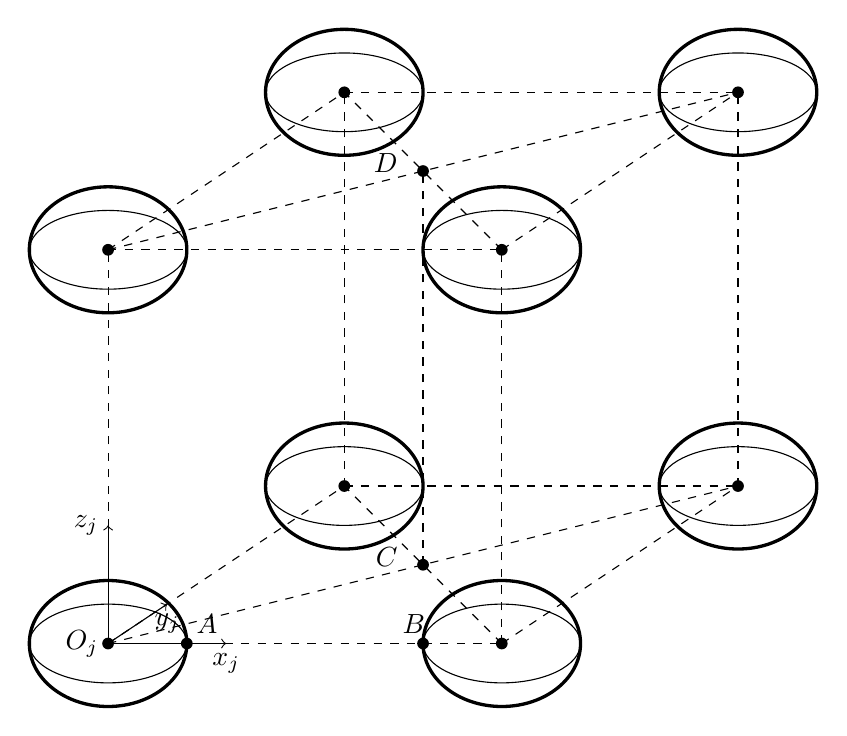
\begin{tikzpicture}%[scale=1.5]
\draw[->] (0,0) -- (1.5,0) node[anchor=north] {$x_j$};
\draw[->] (0,0) -- (0,1.5) node[anchor=east] {$z_j$};
\draw[->] (0,0) -- (0.75,0.5) node[anchor=north] {$y_j$};

\node[left] at (0,0) {$O_j$};
\node[above right] at (1,0) {$A$};
\node[above left] at (4.15,0) {$B$};
\node[left] at (3.8,1.1) {$C$};
\node[left] at (3.8,6.1) {$D$};

\draw[very thick] (0,0) ellipse (1.0 and 0.8);
\draw (0,0) ellipse (1.0 and .5);

\draw[very thick] (3,2) ellipse (1.0 and 0.8);
\draw (3,2) ellipse (1.0 and .5);

\draw[very thick] (0,5) ellipse (1.0 and 0.8);
\draw (0,5) ellipse (1.0 and .5);

\draw[very thick] (3,7) ellipse (1.0 and 0.8);
\draw (3,7) ellipse (1.0 and .5);


\draw[very thick] (5,0) ellipse (1.0 and 0.8);
\draw (5,0) ellipse (1.0 and .5);

\draw[very thick] (8,2) ellipse (1.0 and 0.8);
\draw (8,2) ellipse (1.0 and .5);

\draw[very thick] (5,5) ellipse (1.0 and 0.8);
\draw (5,5) ellipse (1.0 and .5);

\draw[very thick] (8,7) ellipse (1.0 and 0.8);
\draw (8,7) ellipse (1.0 and .5);

\draw[dashed] (0,0) -- (0,5);
\draw[dashed] (0,0) -- (5,0);
\draw[dashed] (0,0) -- (3,2);
\draw[dashed] (0,5) -- (3,7);
\draw[dashed] (0,5) -- (5,5);
\draw[dashed] (3,2) -- (3,7);
\draw[dashed] (3,2) -- (8,2);
\draw[dashed] (5,0) -- (5,5);
\draw[dashed] (5,0) -- (8,2);
\draw[dashed] (8,2) -- (8,7);
\draw[dashed] (3,7) -- (8,7);
\draw[dashed] (5,5) -- (8,7);
\draw[dashed] (0,0) -- (8,2);
\draw[dashed] (5,0) -- (3,2);
\draw[dashed] (0,5) -- (8,7);
\draw[dashed] (5,5) -- (3,7);
\draw[dashed] (4,1) -- (4,6);

\node[circle, fill=black, inner sep=1.5pt] at (0,0) {};
\node[circle, fill=black, inner sep=1.5pt] at (3,2) {};
\node[circle, fill=black, inner sep=1.5pt] at (5,0) {};
\node[circle, fill=black, inner sep=1.5pt] at (8,2) {};

\node[circle, fill=black, inner sep=1.5pt] at (0,5) {};
\node[circle, fill=black, inner sep=1.5pt] at (5,5) {};
\node[circle, fill=black, inner sep=1.5pt] at (3,7) {};
\node[circle, fill=black, inner sep=1.5pt] at (8,7) {};

\node[circle, fill=black, inner sep=1.5pt] at (1,0) {};
\node[circle, fill=black, inner sep=1.5pt] at (4,0) {};

\node[circle, fill=black, inner sep=1.5pt] at (4,1) {};
\node[circle, fill=black, inner sep=1.5pt] at (4,6) {};

\end{tikzpicture}
\end{document}

%%% Local Variables: 
%%% mode: latex
%%% TeX-master: t
%%% End: 
